Suppose that we want to study whether students enrolled in a campus wellness program get more sleep than the average college student.  (This problem assumes that the wellness group comes from the same general population as the other college students.)  Suppose that the average student gets 6.1 hours of sleep per day and denote $\mu$ denote the average sleep gotten by a student in the wellness population.
\begin{enumerate}[label=(\alph*)]
    \item State the hypothesis test for the test you are designing.
    \begin{mybox}
        \textbf{Solution: }

        \nl We are testing whether the wellness group gets \textit{more} sleep than the general population. Hence, we are testing $\mu_a > \mu_0$. The null hypothesis is that there is no difference in means, thus $\mu_a = \mu_0$. 
        \begin{align*}
            H_0 &: \mu_0 = \mu_a
            \\ H_a &: \mu_0 < \mu_a
        \end{align*}
    \end{mybox}
\end{enumerate}
Assume the standard \textit{deviation} is known as $\sigma=0.5$ hour and that the underlying sleep distribution is normal and that there are 16 students in the wellness program.  We define the rejection region to be $\bar{Y}>6.3$.
\begin{enumerate}[label=(\alph*)]
    \setcounter{enumii}{1}
    \item Find $\alpha$, the probability of Type I error.
    \begin{mybox}
        \textbf{Solution: }

        \nl We will show the probability that $H_0$ is rejected when it is true. (df = 15)
        \begin{align*}
            \alpha &= \Pr(\text{Type I error})\\
            &= \Pr(\ybar > 6.3 \mid \mu_0 = 6.1)\\
            &= \Pr\pars{t > \frac{6.3-6.1}{0.5 \big/ \sqrt{16}}}\\
            &= \Pr(t > 1.6)\\
            &\approx 0.065223 \tag{By WA \say{technology}}
        \end{align*}
        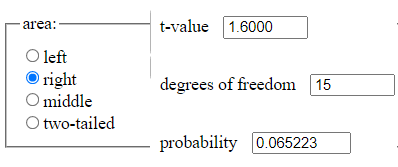
\includegraphics[height=1.5in]{p1b.PNG}
    \end{mybox}
\newpage
    \item Find $\beta$, the probability of Type II error at $\mu=6.3, 6.5,$ and $6.7$.
    \begin{mybox}
        \textbf{Solution: }

        \nl For the probability of a Type 2 error, we want the left tail probability.

        \nl When $\mu = 6.3,$
        $$\mathcal{T}= \frac{\ybar - \mu}{S \big/\sqrt{n}} = \frac{6.3-6.3}{0.5 \big/\sqrt{15}} = 0$$
        And $\Pr(\mathcal{T} < 0) = 0.5$.\\ $\beta = 0.5$ \\\_\_\_\_\_\_\_\_\_\_\_\_\_\_\_\_\_\_\_\_\_\_\_\_\_\_\_\_\_\_\_\_\_\_\_\_\_\_\_\_\_\_\_\_\_\_\_\_\_\_\_\_\_\_\_\_\_\_\_\_\_\_\_\_\_\_\_\_\_\_\_\_\_\_\_\_\_\_\_\_\_\_\_\_\_\_\_\_\_\_\_
        
        
        \nnl When $\mu = 6.5,$
        $$\mathcal{T}= \frac{\ybar - \mu}{S \big/\sqrt{n}} = \frac{6.3-6.5}{0.5 \big/\sqrt{15}} = -1.54919$$
        And $\Pr(Z < -1.54919) \approx 0.071087$.

        \noindent 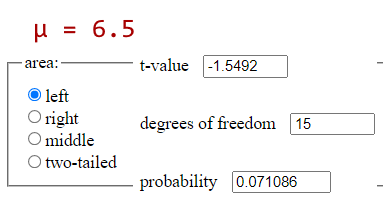
\includegraphics[height=1.5in]{165.PNG}
        \\ $\beta = 0.071087$\\
        \_\_\_\_\_\_\_\_\_\_\_\_\_\_\_\_\_\_\_\_\_\_\_\_\_\_\_\_\_\_\_\_\_\_\_\_\_\_\_\_\_\_\_\_\_\_\_\_\_\_\_\_\_\_\_\_\_\_\_\_\_\_\_\_\_\_\_\_\_\_\_\_\_\_\_\_\_\_\_\_\_\_\_\_\_\_\_\_\_\_\_
        
        \nnl When $\mu = 6.7,$
        $$\mathcal{T}= \frac{\ybar - \mu}{S \big/\sqrt{n}} = \frac{6.3-6.7}{0.5 \big/\sqrt{15}} = -3.09838$$
        And $\Pr(Z < -3.09838) \approx 0.003671$.

        \noindent 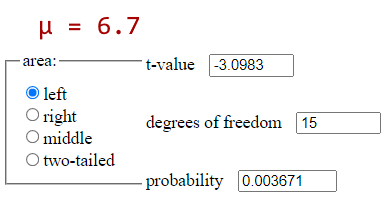
\includegraphics[height=1.5in]{166.PNG}
        \\ $\beta = 0.003671$
    \end{mybox}
    \newpage
    \item Sketch the power function for this test.
    
    \nnl \textbf{Solution: } The following Desmos graph is has the \red{red } line as the power function $\red{\operatorname{power}(\theta) = 1-\beta(\theta)}$. This is approximately the same shape as the respective T distribution with 15 degrees of freedom, but was easier to set up the integral with normal.
    \makeatletter
    \begingroup   %% <- limit scope of the following changes
    \par        %% <- start a new paragraph
    \@totalleftmargin=0pt \linewidth=\columnwidth
    %% ^^ let other commands know that the margins have been reset
    \parshape 0
    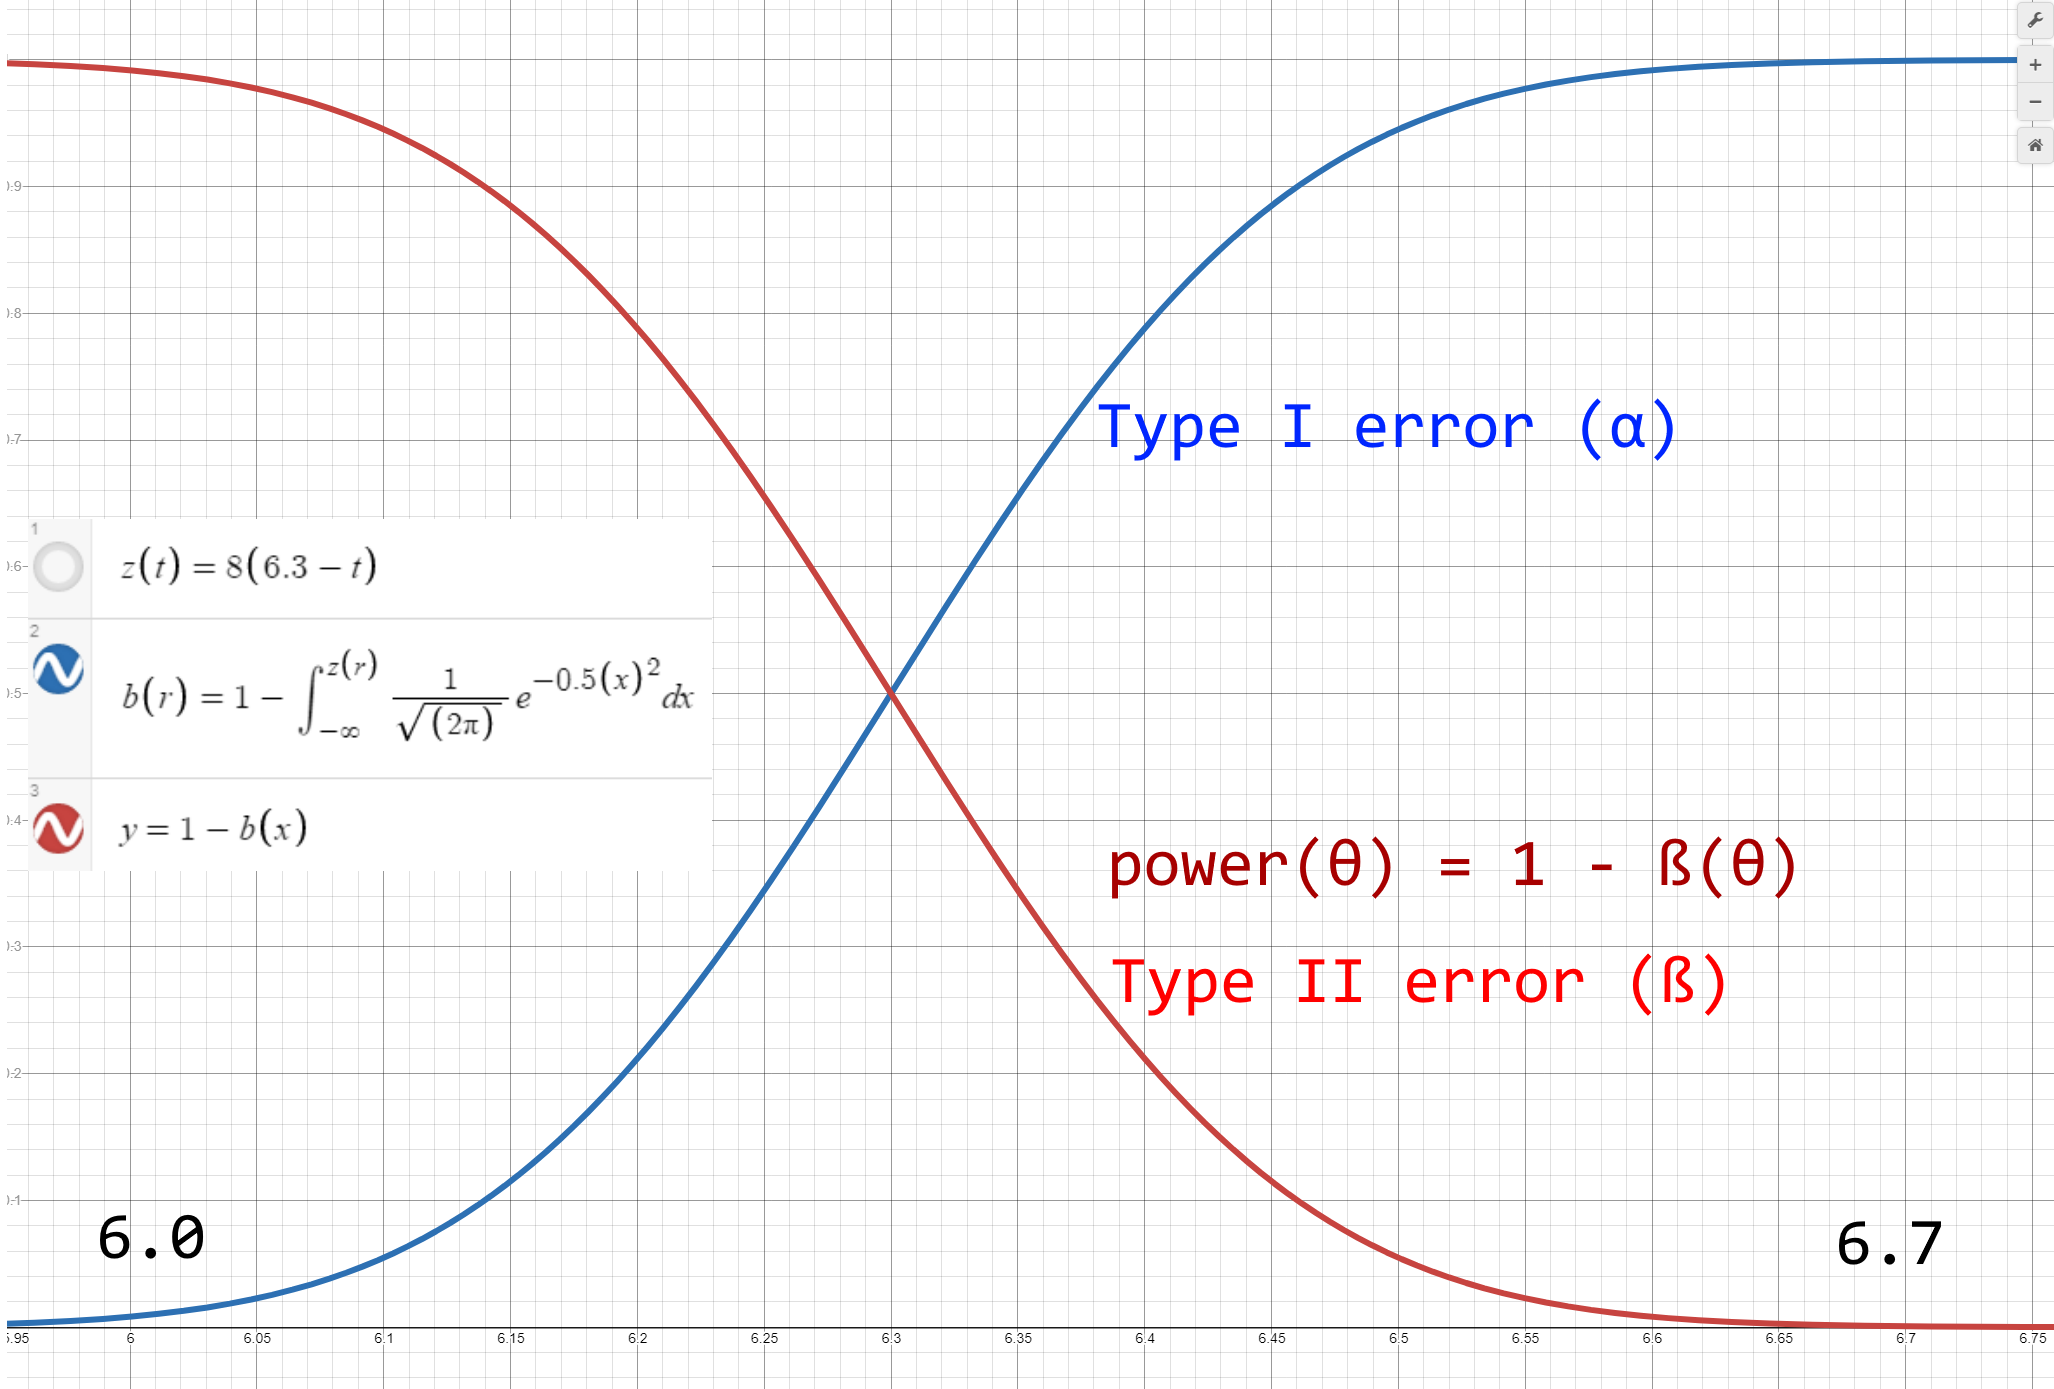
\includegraphics[width=6.5in]{prob1.PNG}
    %% ^^ reset the margins
    \par      %% <- insert #1 and end this paragraph
  \endgroup
    
\end{enumerate}